%
% domain.tex -- graph of characteristics in problem 90000020
%
% (c) 2019 Prof Dr Andreas Müller, Hochschule Rapperswil
%
\documentclass[tikz,12pt]{standalone}
\usepackage{amsmath}
\usepackage{times}
\usepackage{txfonts}
\usepackage{pgfplots}
\usepackage{csvsimple}
\usetikzlibrary{arrows,intersections,math}
\begin{document}
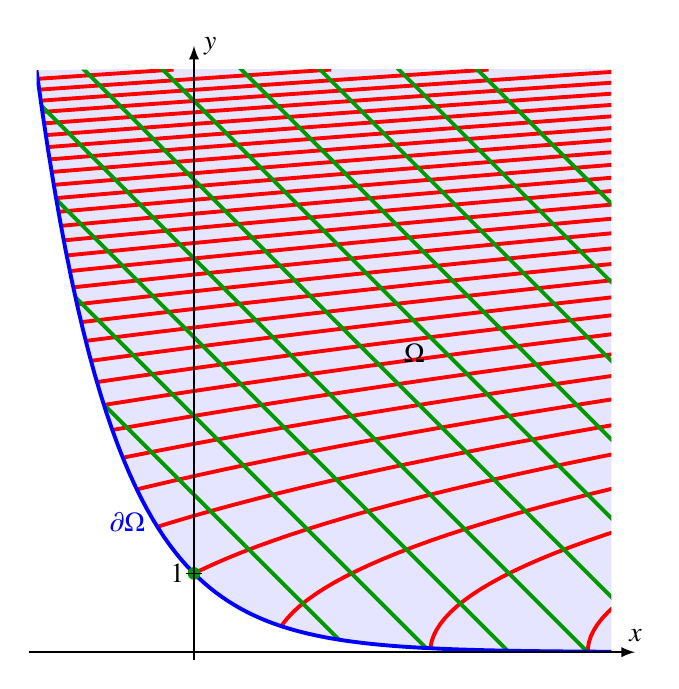
\begin{tikzpicture}[>=latex]

\definecolor{darkgreen}{rgb}{0,0.6,0}

\begin{scope}
\clip (-2.0,-0.0) rectangle (5.3,7.4);

\fill[color=blue!10] plot[domain=-2:5.3,samples=100] ({\x},{exp(-\x)})
	-- (5.4,7.5)--cycle;

\begin{scope}
\clip plot[domain=-2:5.3,samples=100] ({\x},{exp(-\x)})
	-- (5.4,7.5)--cycle;

\foreach \D in {-7,-5,...,55}{
	\draw[color=red,line width=1.4pt]
		plot[domain=-0.1:{7.4},samples=100] ({(\x*\x-\D)},{\x});
}

\foreach \C in {1,...,11}{
	\draw[color=darkgreen,line width=1.4pt]
		({\C},0)--({\C-8},8);
}

\end{scope}

\draw[color=blue,line width=1.4pt]
	plot[domain=-2:5.3,samples=100] ({\x},{exp(-\x)});

\end{scope}

\fill[color=darkgreen] (0,1) circle[radius=0.08];

\draw (-0.1,1)--(0.1,1);

\node at (0,1) [left] {$1$};

\draw[->,line width=0.7pt] (-2.1,0)--(5.6,0) coordinate[label={$x$}];
\draw[->,line width=0.7pt] (0,-0.1)--(0,7.7) coordinate[label={right:$y$}];

\node at (2.8,3.8) {$\Omega$};
\node[color=blue] at (-0.5,{exp(0.5)}) [left] {$\partial\Omega$};

\end{tikzpicture}
\end{document}

